\chapter{Dataset}
\label{chapter:dataset} 


\section{Introduction}

\lipsum[2-4]

\section{Clinical study design}

\lipsum[2-4]

\section{Instrumentation}


\begin{figure}[tbh]
  \centering
  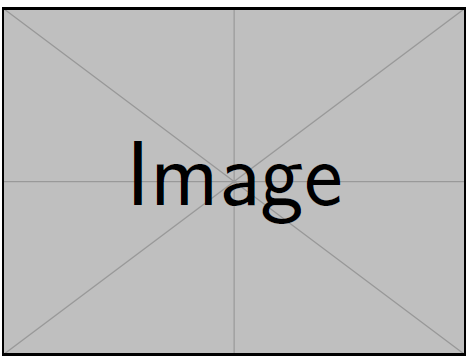
\includegraphics[width=0.9\linewidth,keepaspectratio=true]{dummy_image}
  \caption[Sample image]
  {
  Sample image.
  }
  \label{fig:sample_image}
\end{figure}

\Cref{fig:sample_image} shows the a dummy image ...


\lipsum[2-4]

\begin{figure}[tbh]
  \centering
  \subbottom[]{
    \label{fig:subfig_example:fig1}
    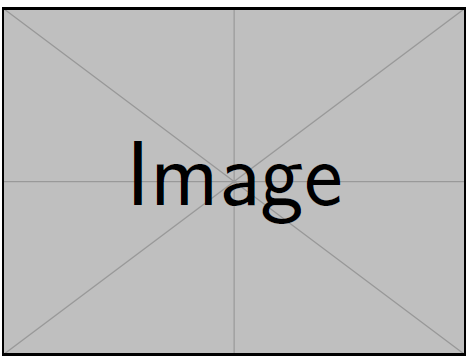
\includegraphics[width=0.3\linewidth,keepaspectratio=true]{dummy_image}
  } 
  \subbottom[]{
    \label{fig:subfig_example:fig2}
    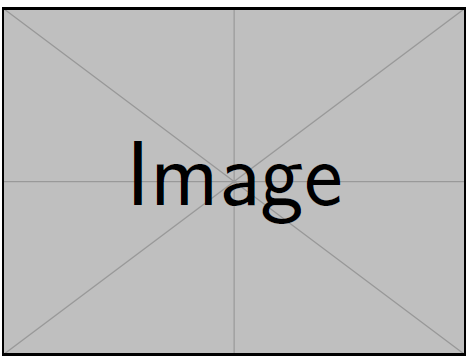
\includegraphics[width=0.3\linewidth,keepaspectratio=true]{dummy_image}
  }
  \subbottom[]{
    \label{fig:subfig_example:fig3}
    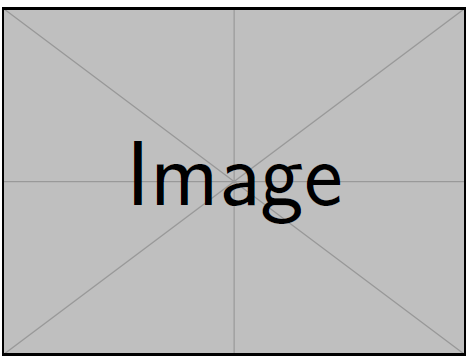
\includegraphics[width=0.3\linewidth,keepaspectratio=true]{dummy_image}
  }
  \caption[The PointGrey Grasshopper2 video camera]
  {
  Caption of the figure, showingy:
  \subcaptionref{fig:subfig_example:fig1} description 1,
  \subcaptionref{fig:subfig_example:fig2} description 2.
  \subcaptionref{fig:subfig_example:fig3} description 3.
  }
  \label{fig:subfig_example}
\end{figure}

\Cref{fig:subfig_example} shows the video camera used in the study ... \cref{fig:subfig_example:fig1} shows ....

\lipsum[2-4]

\Cref{table:camera_specs} describes the ...

\begin{table}[bth]
  \centering
  \caption[General features and specification for the PointGrey Grasshopper2 camera]
  {
  General features and specification for the PointGrey Grasshopper2 camera. (Source: PointGrey)}
  {\small
   \singleTableRowHeight
   \begin{tabular}{ll}
     \tableHeaderStart
        \tableHCell{Item} & \tableHCell{Description} \\
     \tableHeaderEnd
     Imaging Sensor        & Sony ICX625 2/3" progressive scan CCD \\
     Image size (pixels)   & 2448 (H) x 2048 (V)                   \\
     Pixel Size            & 3.45 \si{\micro\metre} x 3.45 \si{\micro\metre} \\
     A/D Converter         & AD9977 14-bit, dual-channel           \\
     Max frame rate        & 15 FPS                                \\
     Video Data Output     & 8, 12, 16 and 24-bit digital data     \\
     Gain \& Exposure                  & Automatic/Manual/One-Push              \\
     Lens Mount            & C-mount                                \\
     Interface             & Gigabit Ethernet                       \\
     Physical dimensions   & 44 (W) mm x 29 (H) mm x 58 (L) mm \\
     \hline 
   \end{tabular}
  }
  \label{table:camera_specs}
\end{table}

\lipsum[2-4]

\section{Patient population}

\lipsum[2-4]


\begin{table}[htb]
  \centering
  \caption{Summary of population demographics in the training and test sets}
  {
    \small
    \begin{tabular}{p{2cm} c c c c c c c c c c}
      \toprule

      Set &
      \multirowcell{2}{Number of\\subjects} &
      \multirowcell{2}{Total time\\(hours)}$^1$ &
      \multicolumn{2}{c}{Gender} &      
      \multicolumn{6}{c}{Ethnicity$^2$}  \\

      \cmidrule{4-11}
        
      &  &  & Male & Female & W & B & A & WB & WA & O  \\
      \midrule
      Training  & 15 & 216.6 & 8  & 7  & 10 & 1   & 1 & 1 & 1 & 1 \\        
      Test      & 15 & 210.0 & 10 & 5  & 10 & $-$ & 1 & 1 & 2 & 1 \\        
      \midrule        
      Total	& 30 & 426.6 & 18 & 12 & 20 & 1   & 2 & 2 & 3 & 2 \\
        
      \bottomrule
        
      \multicolumn{11}{l}
      {
        \footnotesize $^1$ Period during which both reference and estimated data were being recorded simultaneously.        
      } \\        
      \multicolumn{11}{l}
      {        
        \footnotesize $^2$ W = White, B = Black, A = Asian, WB = Mixed White \& Black, WA = Mixed White \& Asian and O = Other.        
      } \\
        
      \end{tabular}      
  } 
  \label{table:patient_demographics}
\end{table}

\subsection{Demographics}

The summary of the demographics for the entire set is described in  \cref{table:patient_demographics}. ...

\lipsum[2-4]

\subsection{Vital signs}

\lipsum[2-4]

\section{Conclusion}

\lipsum[2-4]